\documentclass[lang=cn,newtx,10pt,scheme=chinese]{elegantbook}
\usepackage{realboxes}

\title{ESP32教程}
\author{左元}

\setcounter{tocdepth}{3}

\cover{cover.pdf}

% 本文档命令
\usepackage{array}
\newcommand{\ccr}[1]{\makecell{{\color{#1}\rule{1cm}{1cm}}}}

% 修改标题页的橙色带
\definecolor{customcolor}{RGB}{32,178,170}
\colorlet{coverlinecolor}{customcolor}
\usepackage{cprotect}

\newtcolorbox{marker}[1][]{enhanced,
  before skip=2mm,after skip=3mm,
  boxrule=0.4pt,left=5mm,right=2mm,top=1mm,bottom=1mm,
  colback=yellow!50,
  colframe=yellow!20!black,
  sharp corners,rounded corners=southeast,arc is angular,arc=3mm,
  underlay={%
    \path[fill=tcbcolback!80!black] ([yshift=3mm]interior.south east)--++(-0.4,-0.1)--++(0.1,-0.2);
    \path[draw=tcbcolframe,shorten <=-0.05mm,shorten >=-0.05mm] ([yshift=3mm]interior.south east)--++(-0.4,-0.1)--++(0.1,-0.2);
    \path[fill=yellow!50!black,draw=none] (interior.south west) rectangle node[white]{\Huge\bfseries !} ([xshift=4mm]interior.north west);
    },
  drop fuzzy shadow,#1}

\tcbuselibrary{listings, skins, breakable}
\usepackage[T1]{fontenc}
\usepackage[ttdefault=true]{AnonymousPro}
\definecolor{pblue}{rgb}{0.13,0.13,1}
\definecolor{pgreen}{rgb}{0,0.5,0}

\newtcblisting[auto counter, number within=chapter]{mycode}[1]{
    enhanced,
    attach boxed title to top right={yshift=-\tcboxedtitleheight},
    boxed title style={
        size=small,colback=gray!50,
        colframe=gray!50,
        sharp corners=downhill,
        arc=.5cm,
        top=1mm,bottom=1mm,left=1mm,right=1mm
    },
    fonttitle=\color{black}\itshape\ttfamily,
    colframe=gray!20,
    top=\tcboxedtitleheight,
    bottom=\tcboxedtitleheight,
    sharp corners=downhill,
    arc=.5cm,
    title={#1},
    listing only,
    listing options={
        language=c,
        basicstyle=\fontfamily{AnonymousPro}\selectfont,
        keywordstyle=\bfseries\color{pblue},
        stringstyle=\bfseries\itshape\color{green!40!black},
        commentstyle=\bfseries\itshape\color{black!60},
        % Line numbers
        xleftmargin={0.75cm},
        numbers=left,
        stepnumber=1,
        firstnumber=1,
        numberfirstline=true,
        showspaces=false,
        showtabs=false,
        breaklines=true,
        showstringspaces=false,
        tabsize=1,
        emph={
            downto, for, String, TextView, Toast, Button, EditText, ImageView, Typeface, Intent, WebView, WebSettings, SwipeRefreshLayout, RelativeLayout, Animation, AlertDialog, SharedPreferences, Editor, ToggleButton, CardView, LinearLayout, gradient, shape,
        },
        emphstyle={\bfseries\color{pblue}},
        frame=l
    }
}

\begin{document}

\maketitle
\frontmatter

\tableofcontents

\mainmatter

\chapter{ESP32简介}

ESP32-C3 SoC 芯片支持以下功能:

\begin{itemize}
  \item 2.4 GHz Wi-Fi
  \item 低功耗蓝牙
  \item 高性能 32 位 RISC-V 单核处理器
  \item 多种外设
  \item 内置安全硬件
\end{itemize}

ESP32-C3 采用 40 nm 工艺制成,具有最佳的功耗性能、射频性能、稳定性、通用性和可靠性,适用于各种应用场景和不同功耗需求。

此芯片由乐鑫公司开发。

\begin{marker}
  我们使用的芯片是 ESP32-C3 。
\end{marker}

\chapter{安装开发工具ESP-IDF}

ESP-IDF 需要安装一些必备工具,才能围绕 ESP32-C3 构建固件,包括 Python、Git、交叉编译器、CMake 和 Ninja 编译工具等。

在本入门指南中,我们通过 \textcolor{red}{命令行} 进行有关操作。

\begin{marker}
限定条件:

\begin{itemize}
\item 请注意 ESP-IDF 和 ESP-IDF 工具的安装路径不能超过 90 个字符,安装路径过长可能会导致构建失败。
\item Python 或 ESP-IDF 的安装路径中一定不能包含空格或括号。
\item 除非操作系统配置为支持 Unicode UTF-8,否则 Python 或 ESP-IDF 的安装路径中也不能包括特殊字符(非 ASCII 码字符)
\item 各种路径中不要有中文!
\end{itemize}

系统管理员可以通过如下方式将操作系统配置为支持 Unicode UTF-8:控制面板-更改日期、时间或数字格式-管理选项卡-更改系统地域-勾选选项 “Beta:使用 Unicode UTF-8 支持全球语言”-点击确定-重启电脑。
\end{marker}

\section{离线安装ESP-IDF}

点击\href{https://dl.espressif.com/dl/esp-idf/?idf=4.4}{链接}下载离线安装包。

\begin{figure}[!htb]
\centering

\includegraphics[width=0.9\textwidth]{1.png}
\caption{离线安装包}
\end{figure}

\section{安装内容}

安装程序会安装以下组件:

\begin{itemize}
\item 内置的 Python
\item 交叉编译器
\item OpenOCD
\item CMake 和 Ninja 编译工具
\item ESP-IDF
\end{itemize}

安装程序允许将程序下载到现有的ESP-IDF目录。

推荐将ESP-IDF下载到 \Colorbox{lightgrey}{\lstinline{%userprofile%\Desktop\esp-idf}}目录下,其中\Colorbox{lightgrey}{\lstinline}代表家目录。

\section{启动ESP-IDF环境}

安装结束时,如果勾选了 \Colorbox{lightgrey}{\lstinline{Run ESP-IDF PowerShell Environment}} 或 \Colorbox{lightgrey}{\lstinline{Run ESP-IDF Command Prompt (cmd.exe)}},安装程序会在选定的提示符窗口启动 ESP-IDF。

Run ESP-IDF PowerShell Environment:

\begin{figure}[!htb]
\centering
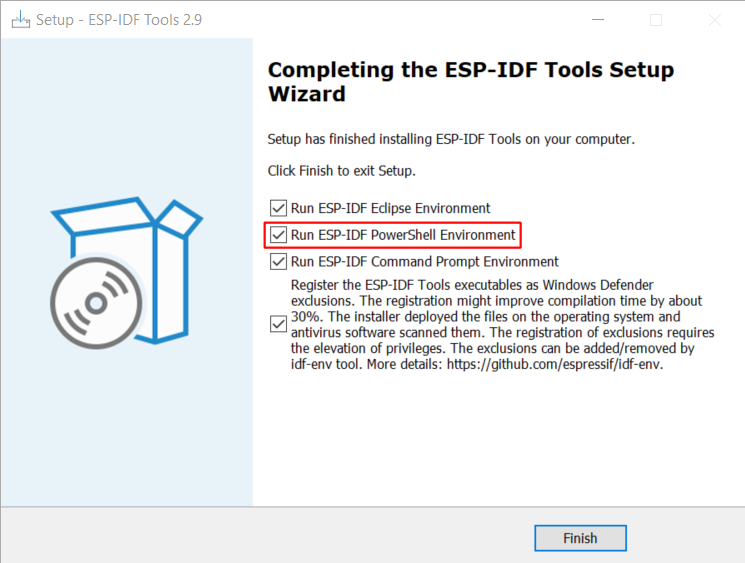
\includegraphics[width=0.9\textwidth]{esp-idf-installer-screenshot-powershell.png}
\caption{PowerShell}
\end{figure}

\chapter{创建工程}

现在,可以准备开发 ESP32 应用程序了。可以从 ESP-IDF 中 examples 目录下的 \Colorbox{lightgrey}{\lstinline{get-started/hello_world}} 工程开始。

\begin{marker}
    ESP-IDF 编译系统不支持 ESP-IDF 路径或其工程路径中带有空格。
\end{marker}

将 \Colorbox{lightgrey}{\lstinline{get-started/hello_world}} 工程复制至本地的 \Colorbox{lightgrey}{\lstinline{~/esp}} 目录下:

\begin{mycode}{复制工程命令}
$ cd %userprofile%\esp
$ xcopy /e /i %IDF_PATH%\examples\get-started\hello_world hello_world
\end{mycode}


\begin{marker}
    ESP-IDF 的 examples 目录下有一系列示例工程,可以按照上述方法复制并运行其中的任何示例,也可以直接编译示例,无需进行复制。
\end{marker}

\end{document}